\section{PID controller (Task 6)}
\label{sec:pd}

A PID controller has been designed so it satisfies the requirements shown in
\autoref{table:pd-requirements} for the cubic polynomial trajectory described
by \autoref{eqn:cubic-trajectory}. The \emph{back-calculation} anti-windup loop
has been implemented. The controller model is shown in \autoref{fig:PID}, the
tuning of the control parameters is described in \autoref{subsec:pid-tuning}
and its behaviour in \autoref{subsec:pid-behaviour}

\begin{figure}
    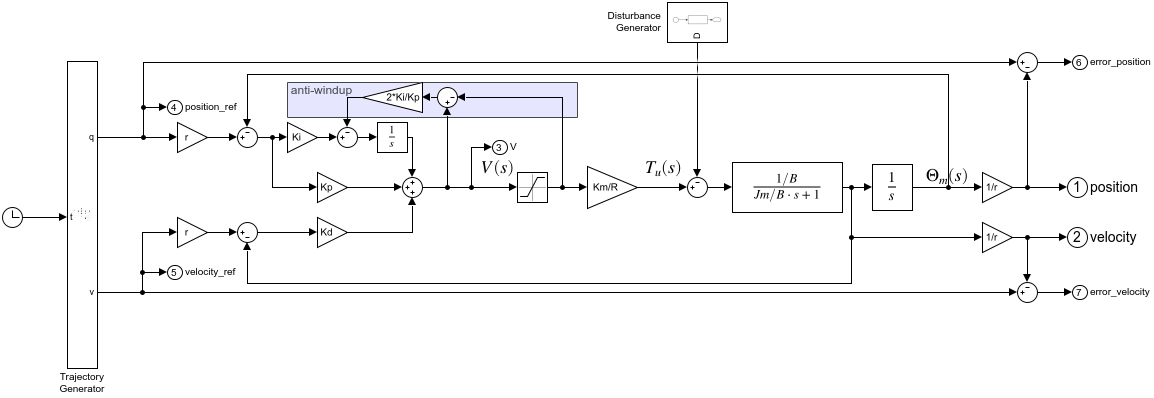
\includegraphics[width=\textwidth]{PID.slx.png}
    \caption{PID controller Simulink model}
    \label{fig:PID}
\end{figure}

\subsection{Tuning}
\label{subsec:pid-tuning}
As in \autoref{subsec:pd-tuning}, a critically damped system is desired and the
speed of the control system $\omega$ is tuned by iterative simulation.

\autoref{table:pid-tuning} shows the different values of the maximal control
error when modifying $\omega$. The value of $\omega = 18$ is therefore chosen to
be used for the rest of the section as it is the lowest value that satisfies
the requirements. The control system gains are calculated as described in
\citetitle{SingleLink} \cite{SingleLink} and the selected anti-windup gain is
$K=2*K_i/K_p$. A bit higher than the recommended as the critically dampening
behaviour is desired, avoiding in this way overshooting. All the gains are
summarized in \autoref{table:pid-constants}.

It is worth to mention that PID control has significantly lower $K_p$ and
$K_d$ gains for the same maximal error requirement.

\begin{table}
    \centering
    \begin{tabular}{c | c}
        $\omega$ & Maximal control error \\ \hline\hline
        $20$ & $0.007152$ \\ \hline
        $18$ & $0.009417$ \\ \hline
        $17$ & $0.011001$ \\ \hline
        $15$ & $0.015163$ \\ \hline
    \end{tabular}
    \\ [1ex]
    \caption{PID controller tuning}
    \label{table:pid-tuning}
\end{table}

\begin{table}
    \centering
    \begin{tabular}{c | c}
        Variable & Value \\ \hline\hline
        $\omega$ & $18$ \\ \hline
        $K_p$ & $4.291611$ \\ \hline
        $K_d$ & $0.130528$ \\ \hline
        $K_i$ & $25.749669$ \\ \hline
        $K_{anti-windup}$ & $12$ \\ \hline
    \end{tabular}
    \\ [1ex]
    \caption{PID controller parameters}
    \label{table:pid-constants}
\end{table}

\subsection{Behaviour}
\label{subsec:pid-behaviour}
The behaviour of the PID control system has been checked for the step change of
constant reference trajectory from $0$ to $0.5\text{ rad}$ as shown in
\autoref{fig:PID_step}. We obtain the expected damped response,
ensured by our selected anti-windup gain. During the simulations, it was proven
that a lower anti-windup gain resulted in an appreciable overshoot.

\begin{figure}
    \centering
    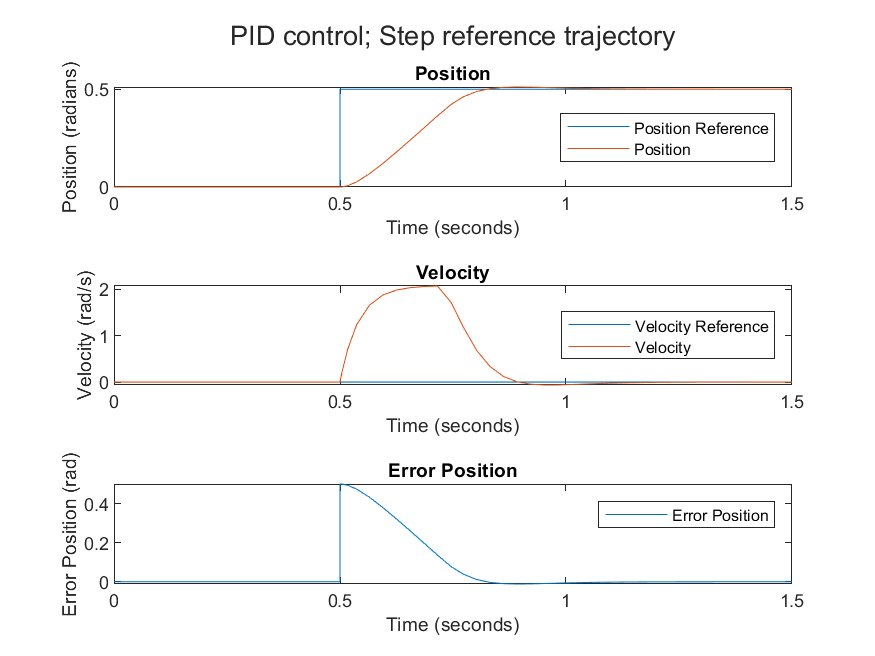
\includegraphics[width=.7\textwidth]{PID_step.png}
    \caption{Behaviour of the PID control system for the step change of constant reference trajectory from $0$ to $0.5\text{ rad}$}
    \label{fig:PID_step}
\end{figure}

\subsubsection{Undisturbed}
The response of the PID control system has been also tested for the cubic
reference trajectory described by \autoref{eqn:cubic-trajectory} and the LSPB
reference trajectory described by \autoref{eqn:LSPB-trajectory}. The results
are shown in \autoref{fig:PID_cubic} and \autoref{fig:PID_LSPB}, respectively.

Unlike in the analogous PD scenario described in
\autoref{subsubsec:pd-undisturbed}, LSPB trajectory shows a greater error than
cubic polynomial. Even with a lower anti-windup gain. Which proves that an
optimal trajectory will depend greatly on the control system.

\begin{figure}
    \centering
    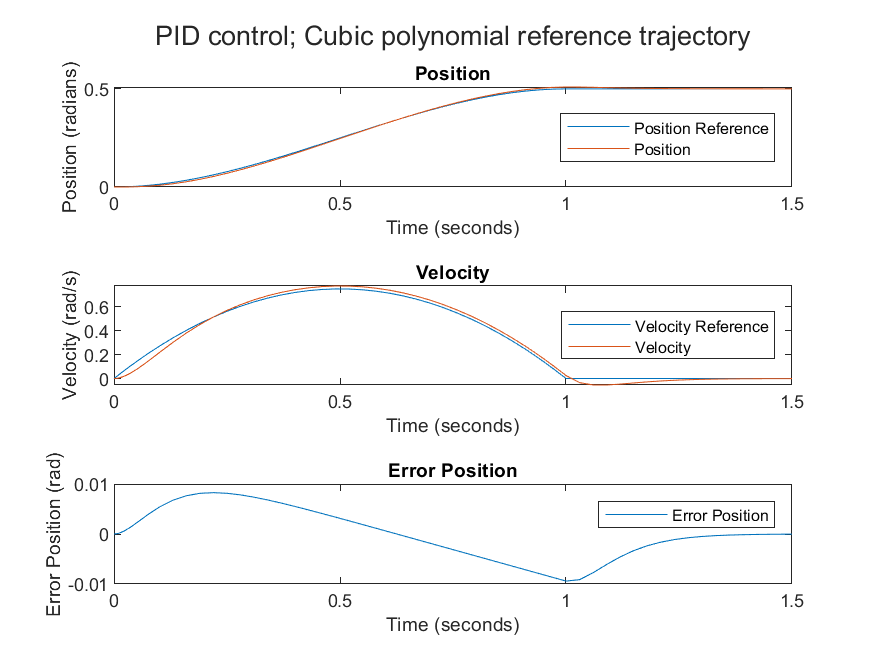
\includegraphics[width=.7\textwidth]{PID_cubic.png}
    \caption{PID control system response for the cubic polynomial trajectory. Error position is the difference between the position reference and the recorded arm position. Being positive when the reference position is greater than the recorded one, negative otherwise.}
    \label{fig:PID_cubic}
\end{figure}

\begin{figure}
    \centering
    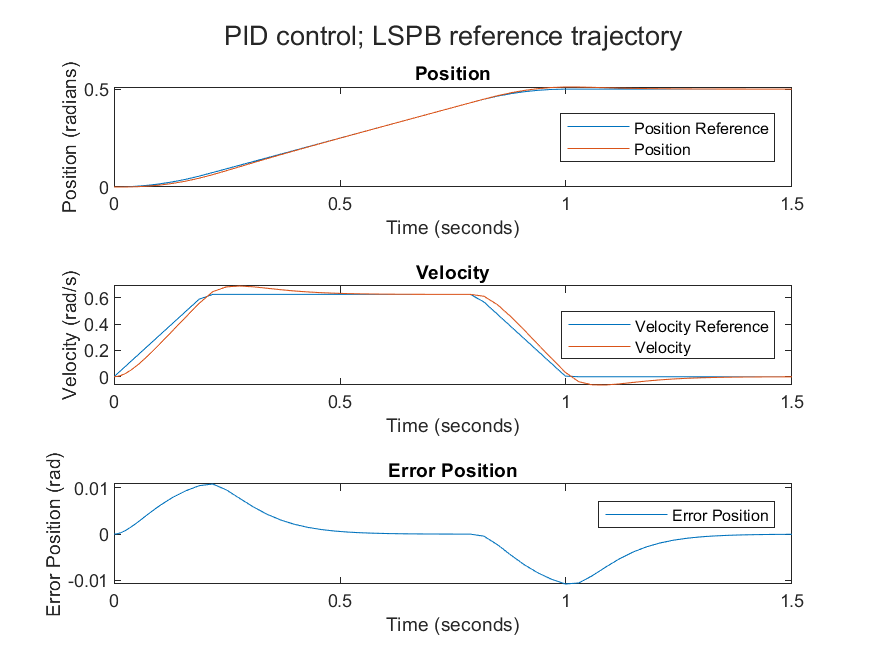
\includegraphics[width=.7\textwidth]{PID_LSPB.png}
    \caption{PID control system response for the LSPB trajectory. Error position is the difference between the position reference and the recorded arm position. Being positive when the reference position is greater than the recorded one, negative otherwise.}
    \label{fig:PID_LSPB}
\end{figure}

\subsubsection{Disturbed}
The response of the PID control system has been tested again in a disturbed
scenario with the two reference trajectories already mentioned. The load
disturbance tested is equal to $\tau_l/r = 2 N\cdot m$ as in
\autoref{subsubsec:pd-disturbed}. \autoref{fig:PID_cubic_disturbed} shows the
results for the cubic polynomial trajectory and
\autoref{fig:PID_LSPB_disturbed} shows the results for the LSPB trajectory.

Unlike again in the analogous PD scenario described in
\autoref{subsubsec:pd-undisturbed}, the steady state error is effectively $0$
with PID control.

\begin{figure}[h]
    \centering
    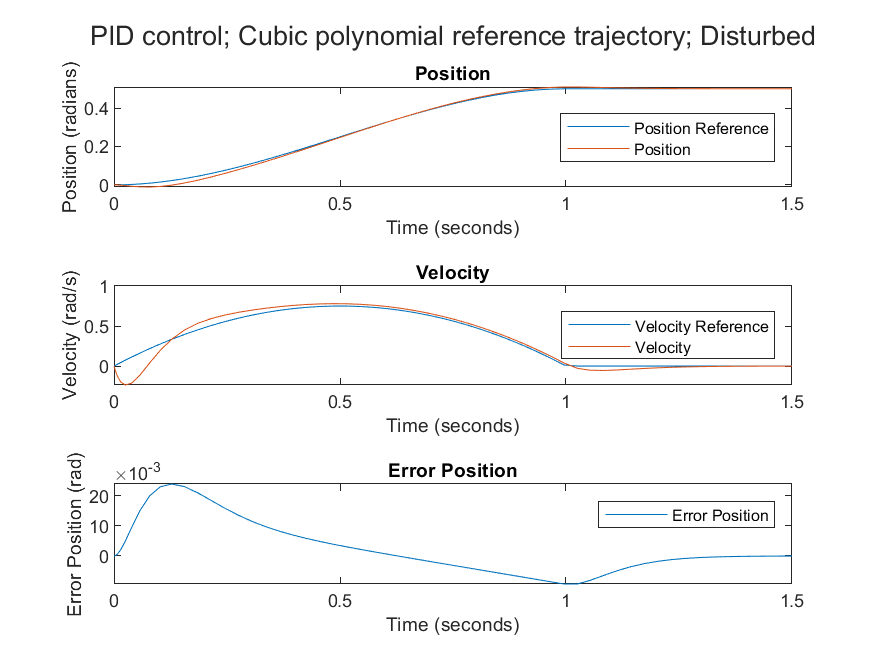
\includegraphics[width=.7\textwidth]{PID_cubic_disturbed.png}
    \caption{PID control system response for the cubic polynomial trajectory
    with disturbance. Error position is the difference between the position reference and the recorded arm position. Being positive when the reference position is greater than the recorded one, negative otherwise.}
    \label{fig:PID_cubic_disturbed}
\end{figure}

\begin{figure}[h]
    \centering
    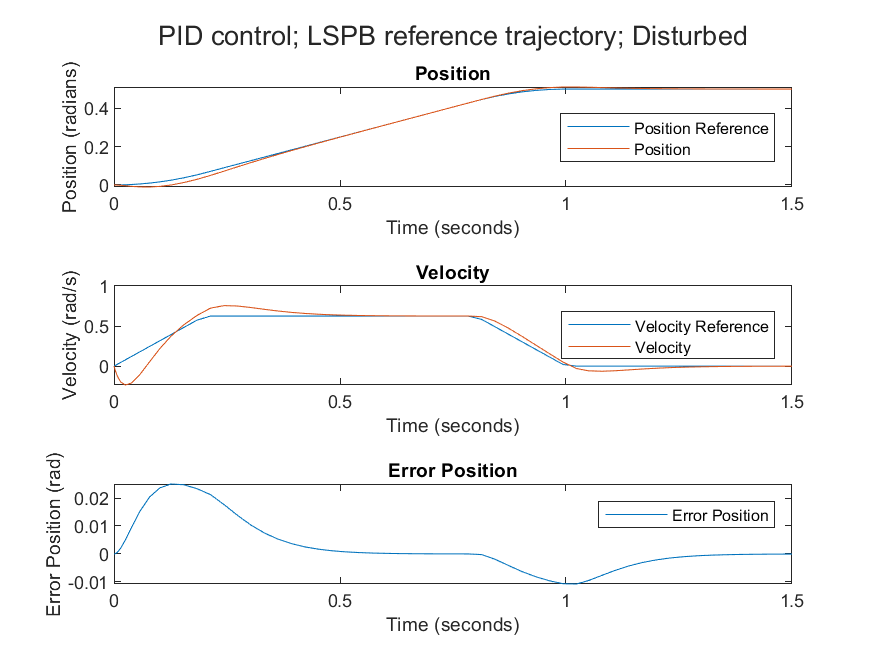
\includegraphics[width=.7\textwidth]{PID_LSPB_disturbed.png}
    \caption{PID control system response for the LSPB trajectory with disturbance. Error position is the difference between the position reference and the recorded arm position. Being positive when the reference position is greater than the recorded one, negative otherwise.}
    \label{fig:PID_LSPB_disturbed}
\end{figure}

\clearpage
\subsection{Feedforward (Task 7)}
Finally, the effect of the feedforward action has been tested for the
sinusoidal reference trajectory described in
\autoref{eqn:sinusoidal-trajectory}. 

\begin{equation}
    \text{Sinusoidal trajectory } q(t) = 0.25*\sin\left(\pi*6.8\right)
    \label{eqn:sinusoidal-trajectory}
\end{equation}

\autoref{fig:PIDfeedforward} illustrates the model of the PID control system
with feedforward action that was used for the simulations.
\autoref{fig:PIDfeedforward_sinusoidal} shows the comparison of using
feedforward action against not using it.

One can realize at first sight that the control system with feedforward action
has a lower error than the one without it. With a closer look one can also see
that both with and without feedforward action steady state trajectories have
the same sinusoidal amplitude and frequency. But the phase of the control
system with feedforward action is better aligned with the reference trajectory.
Which is the cause for the lower error.

Additionally, the control system with feedforward action did not
suffer the same transient state that can be observed in the control system
without feedforward, where the error is even higher. This means that the
feedforward effect will be even more important with random oscillations like
noise in the reference trajectory.

\begin{figure}
    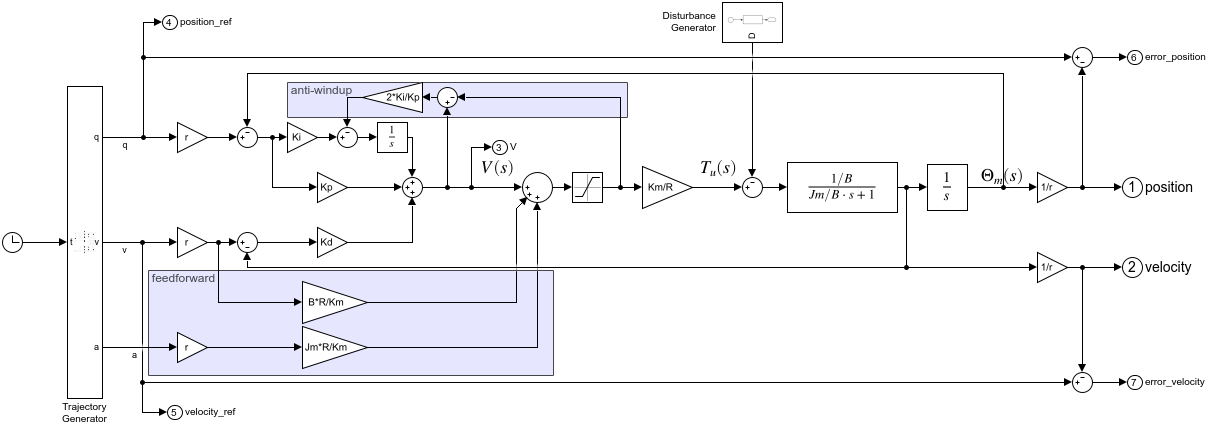
\includegraphics[width=\textwidth]{PIDfeedforward.slx.png}
    \caption{PID controller with feedforward Simulink model}
    \label{fig:PIDfeedforward}
\end{figure}

\begin{figure}[h]
    \centering
    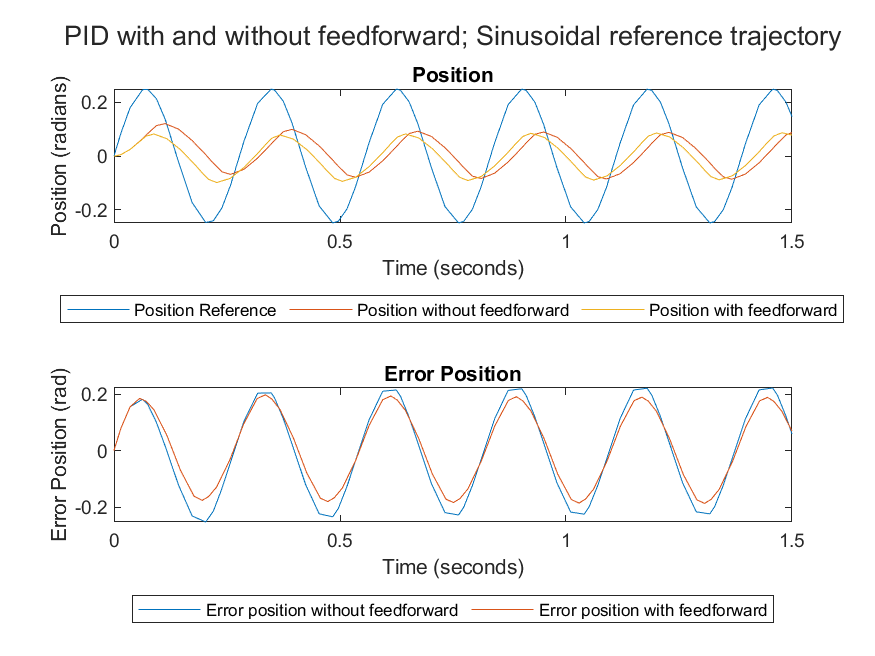
\includegraphics[width=.7\textwidth]{PIDfeedforward_sinusoidal.png}
    \caption{PID control response with and without feedforward action for a sinusoidal trajectory. Error position is the difference between the position reference and the recorded arm position. Being positive when the reference position is greater than the recorded one, negative otherwise.}
    \label{fig:PIDfeedforward_sinusoidal}
\end{figure}